\documentclass{article}

\usepackage{graphics}
\usepackage{color}
\usepackage{verbatim}
\usepackage{amsthm}
\usepackage{amsmath}
\usepackage{amssymb}
\usepackage{graphicx}
\usepackage{esint}
\usepackage{tikz}
\usetikzlibrary{bayesnet}

\begin{document}
\thispagestyle{empty}
\centering
%\missingfigure{Factor graph for binary logistic regression. Just imagine by yourself for now.}
%\includegraphics[scale=0.8,page=2,clip,trim=8cm 18.5cm 8cm 1cm]{img/heess_passing_ep_supp.pdf}
%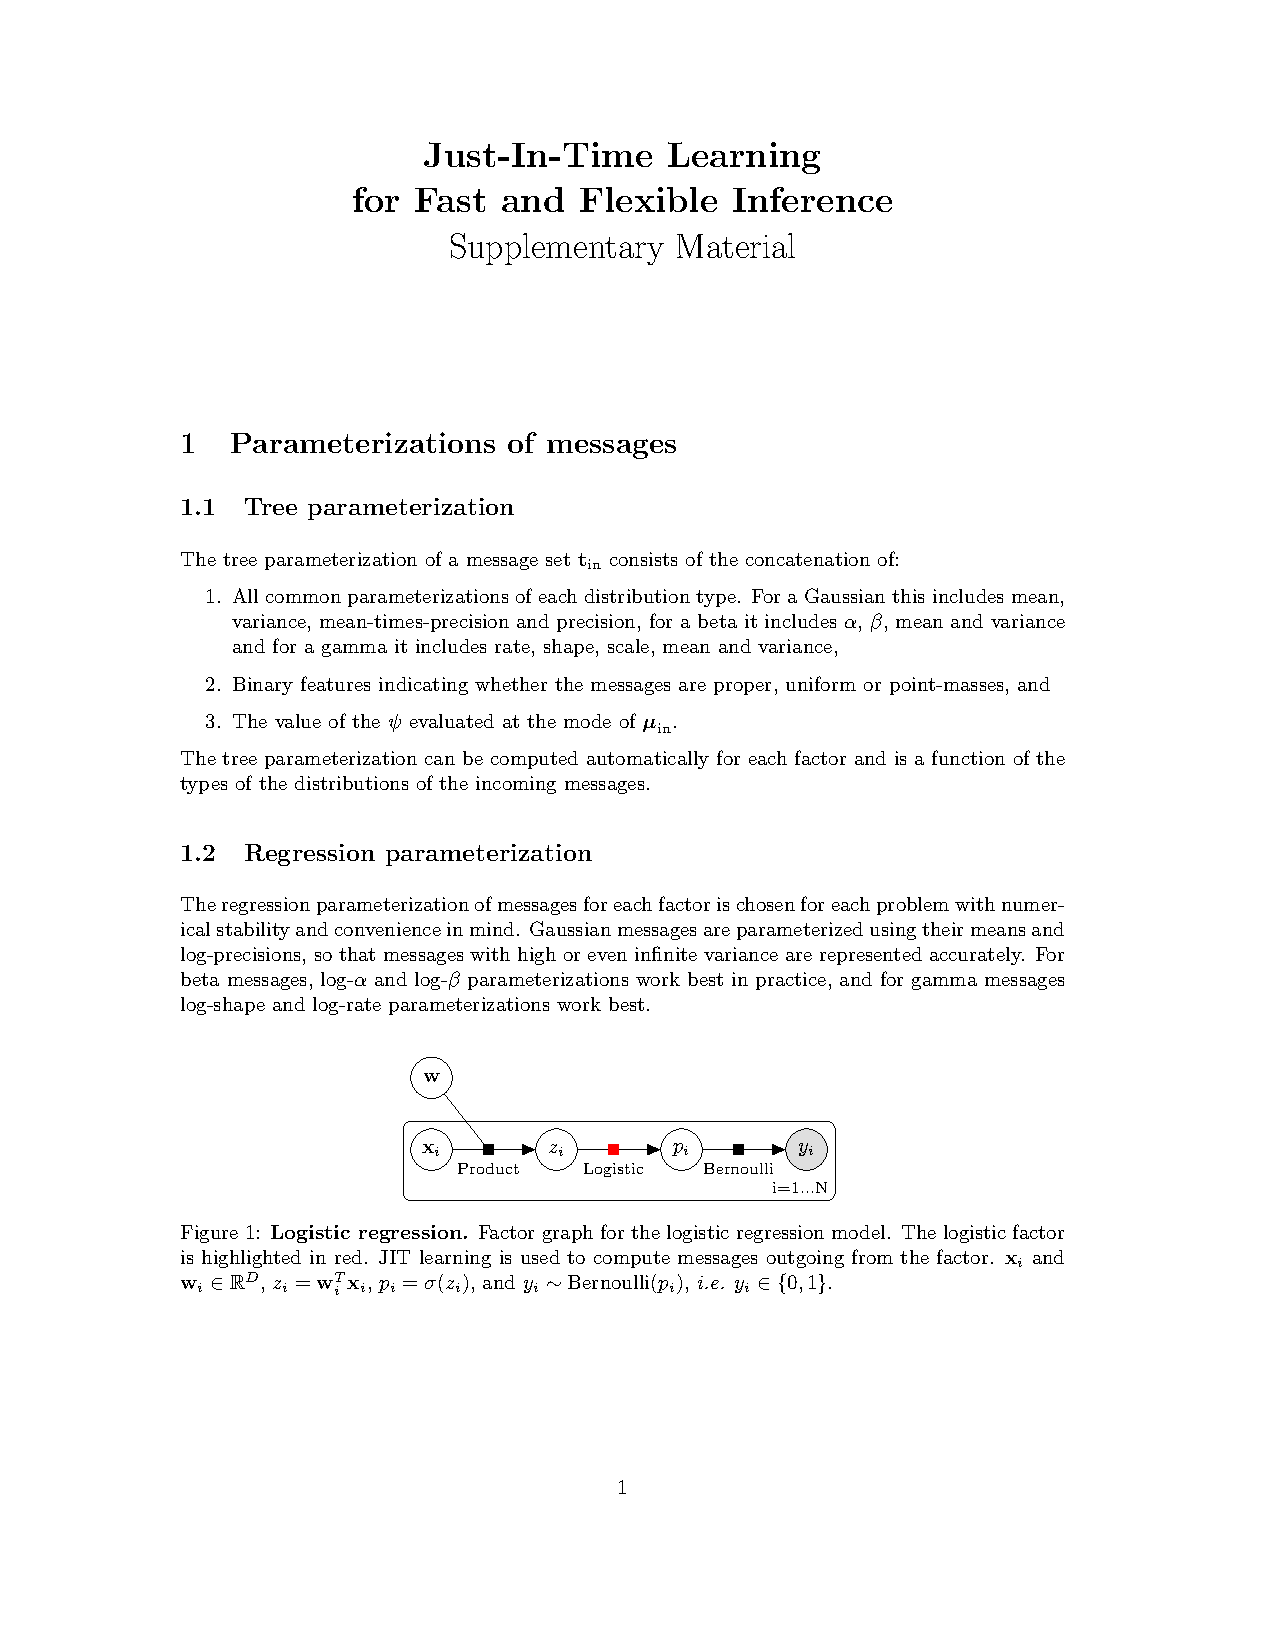
\includegraphics[scale=0.8,page=1,clip,trim=6.5cm 7.5cm 7cm 17.8cm]{img/eslami_jit_supp.pdf}

%vertical
%\begin{tikzpicture}
%    \bayesfactor[color=red] {cg} {above:CG $(f)$} {} {};
%    \node[latent, right = 4mm of cg] (tau) {$\tau$};
%    \bayesfactor[below = 4mm of tau] {gauss} {left:$\mathcal{N}(x_i; 0, \tau) $} {} {};
%    \node[obs, below = 4mm of gauss] (x) {$x_i$};

%    \edge[-] {cg} {tau};
%    \edge[-] {tau} {gauss};
%    \edge[-] {gauss} {x};

%    \plate {sample} {
%       (x)
%   } {$i=1, \ldots, N$};

%\end{tikzpicture}


%horizontal
\begin{tikzpicture}
    \bayesfactor[color=red] {cg} {right:CG $(f)$} {} {};
    \node[latent, below = 4mm of cg] (tau) {$\tau$};
    \bayesfactor[right = 5mm of tau] {gauss} {below:$\mathcal{N}(0, \tau^{-1}) $} {} {};
    \node[obs, right = 17mm of gauss] (x) {$x_i$};

    \edge[-] {cg} {tau};
    \edge[-] {tau} {gauss};
    \edge[-] {gauss} {x};

    \plate {sample} {
       (x)
   } {$i=1, \ldots, N$};

\end{tikzpicture}
\end{document}
